\documentclass{paper}
\usepackage[margin=0.5in]{geometry}
\usepackage{graphicx}
\title{1. Cache}
\begin{document}
\maketitle
\begin{large}\textbf{Hvad er et memory hieraki?} \end{large}
%\renewcommand{\labelitemi}{$\bullet$}
\begin{itemize}

	\item Hvilken memory er tjekket foerst?
	\begin{itemize}
		\item L1, L2, L3, RAM, Devices(Lagringsmedium)
	\end{itemize}
	\item L1 er taettest paa CPU'en, men mindst
	\item L2 er langsommere, men stoerre
	\item L3(hvis tilstede) er endnu langsommere, men ogsaa tilsvarende stoerre
	\item RAM er stoerst, men langsomt
	\item RAM er ogsaa kaldet \textbf{Main Memory}
	\item Eksterne devices(som HDD) er \textbf{Secondary Memory}

\end{itemize}

\begin{large}\textbf{Hvad er cache, og hvad bruger vi den til?} \end{large}

\begin{large}\textbf{Hvordan er en cache opbygget?} \end{large}

\begin{large}\textbf{Hvilke begraensninger har en cache og hvordan kan vi minimere disse?} \end{large}

\begin{large}\textbf{Hvordan kan man som programmoer optimere brugen af cache?} \end{large}

%memory hieraki
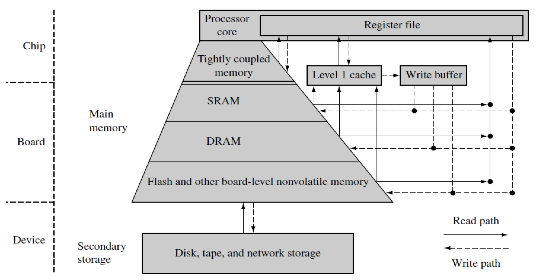
\includegraphics[scale=0.7]{cache.png}
%cache controller

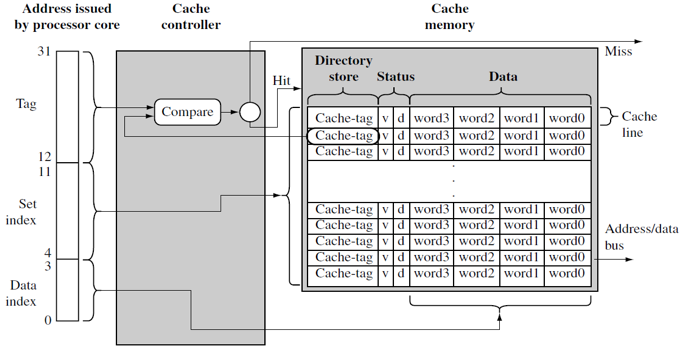
\includegraphics[scale=0.7]{cachecontroller.png}
\end{document}
